\documentclass{article}
\usepackage[T1]{fontenc}
\usepackage{lmodern}
\usepackage{graphicx}
\usepackage{amsmath,amssymb}
\usepackage[a4paper,margin=2cm]{geometry}
\usepackage[absolute,overlay]{textpos}
\setlength{\TPHorizModule}{1mm}
\setlength{\TPVertModule}{1mm}
\usepackage[indonesian]{babel}
\usepackage{hyperref}
\setlength{\emergencystretch}{2em}
% unit: Halaman 26

\begin{document}

% === Halaman 26 (llm) ===

\vspace{121.77mm}

\section*{Diagram Umum \textit{Cipher} alir}

\vspace{60mm}

\begin{itemize}
    \item Bit-bit aliran kunci untuk enkripsi/dekripsi disebut \textit{keystream}
    \item \textit{Keystream} dibangkitkan oleh \textit{keystream generator} berdasarkan umpan (\textit{seed}) U.
    \item Enkripsi dan dekripsi dengan \textit{cipher} alir komputasinya sederhana dan cepat
    \item \textit{Keystream} $c_1, c_2, \dots$ di-XOR-kan dengan aliran bit-bit plainteks, $p_1, p_2, \dots$, menghasilkan aliran bit-bit cipherteks $c_1, c_2, \dots$:
    \[ c_i = p_i \oplus k_i \]
    \item Di sisi penerima dibangkitkan \textit{keystream} yang sama untuk mendekripsi aliran bit-bit cipherteks $c_1, c_2, \dots$ menjadi plainteks, $p_1, p_2, \dots$:
    \[ p_i = c_i \oplus k_i \]
\end{itemize}

% deskripsi: Diagram blok sistem Cipher Alir yang menunjukkan proses enkripsi oleh pengirim dan dekripsi oleh penerima menggunakan Keystream Generator dan operasi XOR.
% bbox normalisasi: [0.2400, 0.1000, 0.8200, 0.5100]
\begin{textblock*}{121.80mm}(50.40mm,29.70mm)
\noindent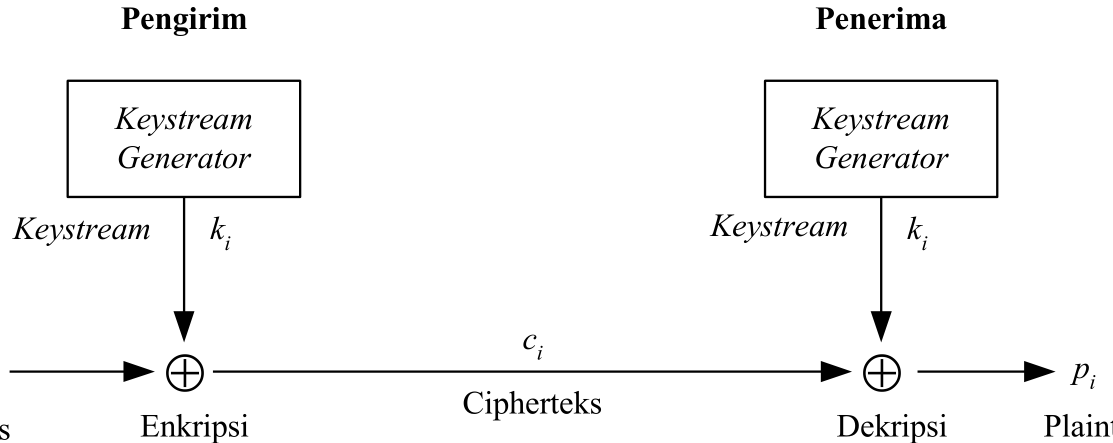
\includegraphics[width=121.80mm,height=121.77mm]{../../images/llm/page_026_img_01.png}%
\end{textblock*}

\end{document}
